\section{Tests de robustesse}
\label{sec:robustness}
% =====================================================================

Nous testons la sensibilité des mesures aux choix numériques sur les 8 premiers sous-volumes du catalogue fiduciel (ligne de visée $z$). Chaque test est répété pour les deux méthodes, et le changement des monopôles des corrélations croisées Q1 et Q4 est exprimé en unités de l'erreur statistique d'un sous-volume (Figure~\ref{fig:robustness}).

\paragraph{Extension périodique.} Augmenter l'extension autour de chaque sous-volume de 30 à $60\Mpch$ laisse inchangées les valeurs ASTRA de $r$, et donc toutes les statistiques : le voisinage de Delaunay de chaque point du sous-volume est déjà contenu dans l'extension de $30\Mpch$.

\paragraph{Nombre de points aléatoires.} Doubler le nombre de points aléatoires dans la tessellation ($N_r=2N_g$) décale les corrélations croisées Q1 d'ASTRA jusqu'à $4\sigma$ et celles de Q4 jusqu'à $2\sigma$ à $s\lesssim40\Mpch$, alors que le density split, pour lequel les points aléatoires ne sont que des points de requête, change de moins de $0.2\sigma$. Dans ASTRA, les points aléatoires entrent dans la définition même de $r$ (Éq.~\ref{eq:astra_r}), donc $N_r/N_g$ est un paramètre de la statistique et doit rester fixé.

\paragraph{Densité d'échantillonnage.} Éclaircir aléatoirement les galaxies (et les points aléatoires dans la même proportion) d'un facteur 2 (5) décale les corrélations croisées d'ASTRA de 7--8 (22)$\sigma$ à $s\simeq20$--$40\Mpch$, et jusqu'à 12 (40)$\sigma$ pour le Q1 des galaxies, contre $\sim1$ (3--5)$\sigma$ pour le density split. Au niveau des points individuels, la corrélation de rang entre les $r$ des mêmes galaxies calculés dans les échantillons complet et éclairci n'est que de $0.65$, $0.38$ et $0.24$ pour des facteurs d'éclaircissement de 2, 5 et 10, et seuls 58\%, 43\% et 36\% des galaxies des quartiles extrêmes conservent leur quartile.

Il s'agit d'une propriété intrinsèque de l'estimateur plutôt que d'une instabilité numérique. ASTRA est une statistique à \emph{échelle adaptative} : l'environnement d'un point est défini par ses voisins de Delaunay, de sorte que son échelle effective est la distance typique entre voisins, $\propto\bar n^{-1/3}$, et qu'elle change avec la densité d'échantillonnage. L'éclaircissement agrandit cette échelle, ce qui explique que les changements soient concentrés à $s\lesssim50\Mpch$, alors que le density split conserve un rayon de lissage fixe. Ce n'est pas une limitation pour la présente analyse ni pour DESI, puisque la densité est fixée dans les mocks comme dans les données (et dans un émulateur entraîné à cette densité). Cela implique cependant que les statistiques ASTRA doivent être comparées, modélisées et émulées à la même densité numérique et au même rapport aléatoires/galaxies, et que les comparaisons avec le density split doivent être faites à densité égale, comme dans tout cet article.

\begin{figure*}[!tp]
\centering
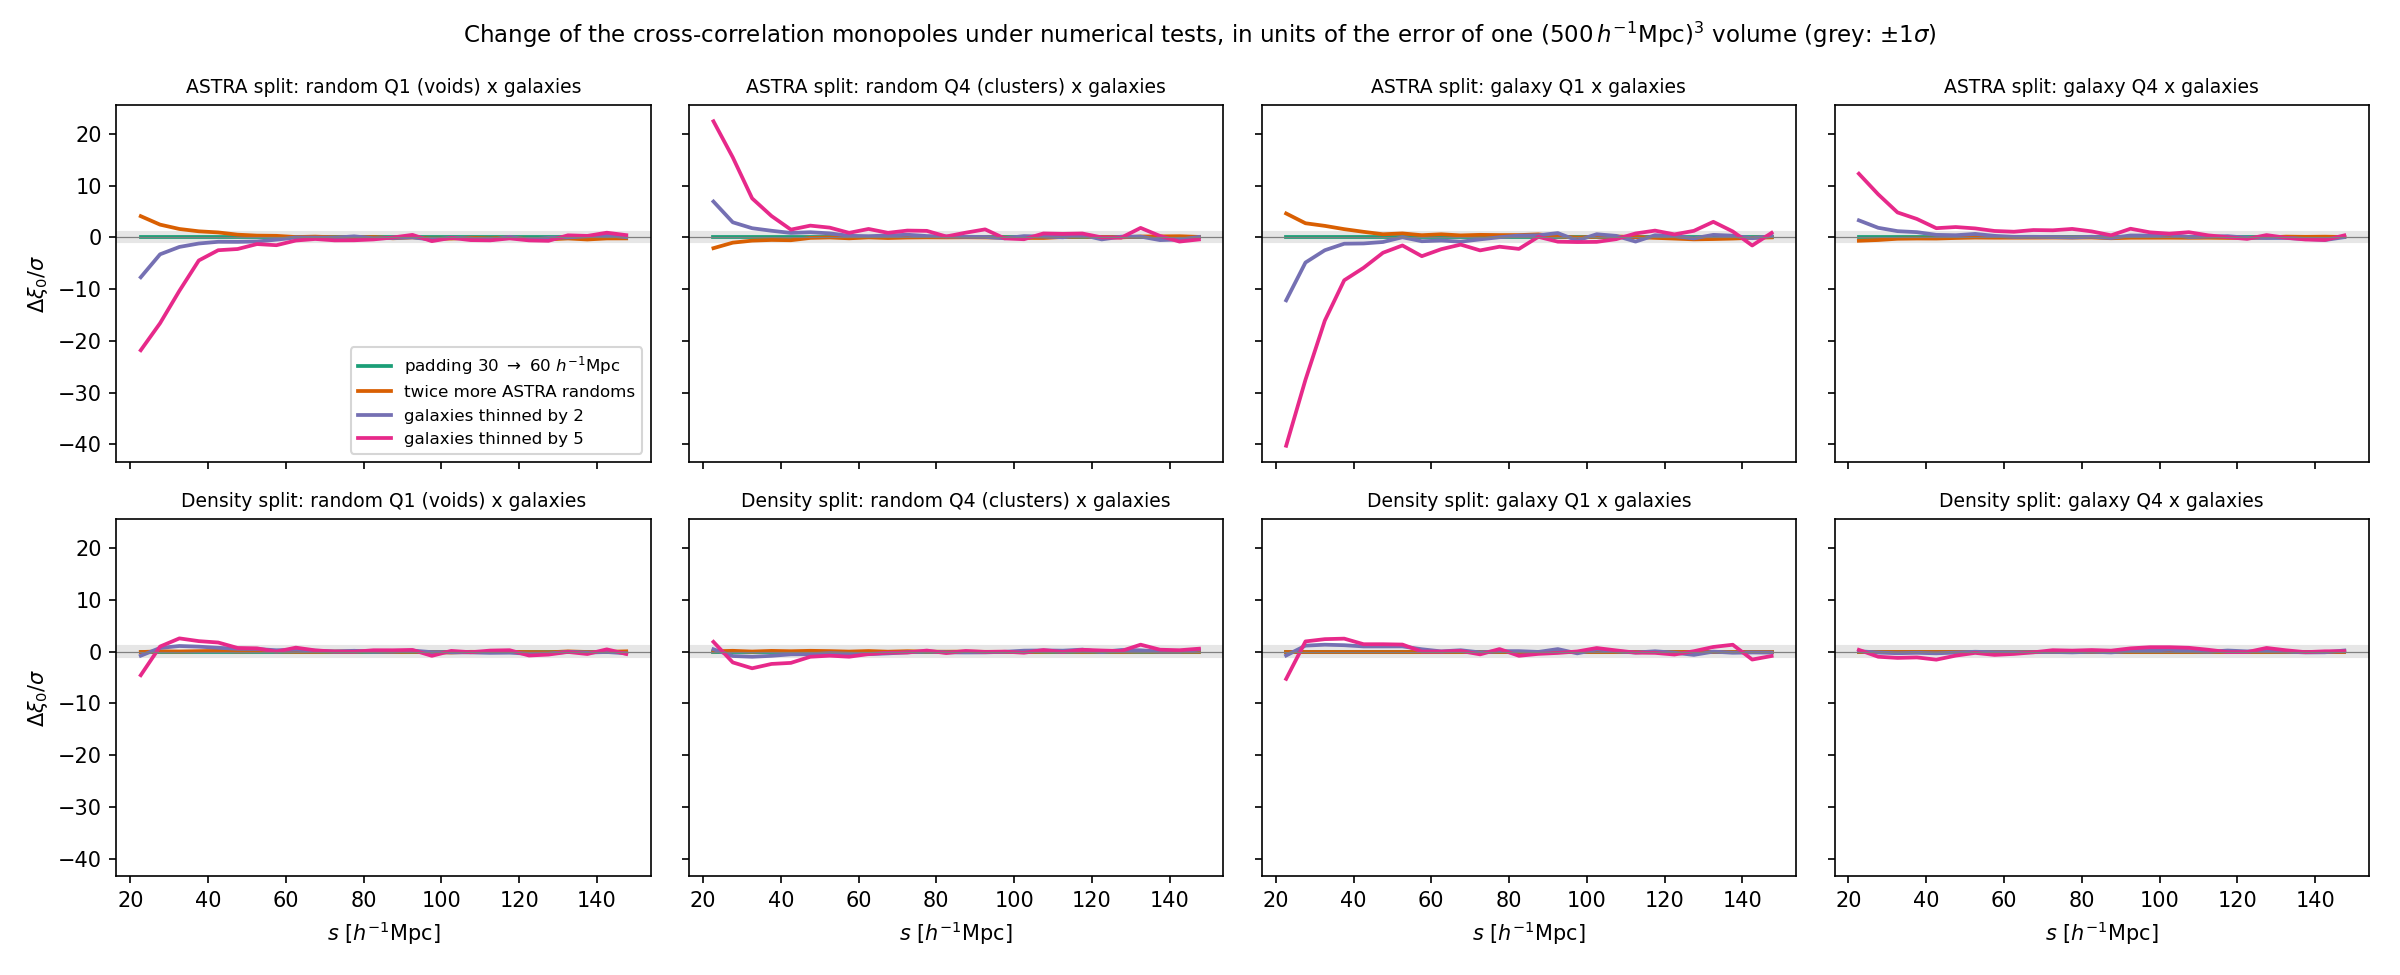
\includegraphics[width=\textwidth]{readable_robustness.png}
\caption{Variation des monopôles des corrélations croisées Q1 et Q4 (quartiles aléatoires, gauche ; quartiles de galaxies, droite) de l'ASTRA split (haut) et du density split (bas) lorsque l'extension est doublée (vert), les points aléatoires d'ASTRA sont doublés (orange), et les galaxies sont éclaircies d'un facteur 2 (violet) et 5 (rose), par rapport à la référence, en unités de l'erreur d'un volume de $(500\Mpch)^3$ (bande grise : $\pm1\sigma$). Moyenne sur 8 sous-volumes du catalogue fiduciel.}
\label{fig:robustness}
\end{figure*}

